% Chapter 2
\chapter{Background Information and Theory} 
\label{Chapter2} 


%----------------------------------------------------------------------------------------
\section{Literature Review} \label{litreview}
% literature review is a paper or article you might sit down to read that gives a general overview of a field. someone not experienced in topic modelling should come a way with a greater understanding of topic models after reading it. And be ready to understand more of your project. 
% explain here what we are going to cover in the literature review.

In this section we begin by reviewing a few of the tasks common in topic modeling. Then we describe a handful of the ways the quality of topic models, LDA in particular, are commonly tested. Finally we discuss the specific tasks of document classification and clustering in the context of topic modeling, as well as the corresponding methods for evaluating model performance at these tasks. 

\subsection{Applications of Topic Modeling}
%------General---------
The most popular application of topic models is simply summarizing large text collections by mining the topics. This is a task LDA is particularly suited for \parencite{griffiths_steyvers04, Mei:2007:ALM:1281192.1281246}. The original LDA paper however \parencite{Blei:2003:LDA:944919.944937} gave promising results on document classification as well. Since then LDA has been used with success not only for document classification, but also for clustering and information retrieval \parencite{Wei:2006:LDM:1148170.1148204, Nagwani2015}. This is due to the strength of the topic vectors LDA models provide, which tend to correlate strongly with human judgement. 

%Though significantly less work has been done assessing the efficacy of LDA extensions such as the DTM and DIM in these areas. 

\subsection{Ensuring Model Quality}
%------Methods of Testing------
\subsubsection{Perplexity Testing}
In order to ensure the strength of these topic vectors researchers employ a handful methods to evaluate the topic models. While the most intuitive method is simply to have humans judge the coherence of each topic, this becomes prohibitively time consuming and expensive for large data sets. One commonly used method of automating this process is by evaluating the topic model on a held out set of testing documents and obtaining the log-likelihood perplexity of the unseen documents \parencite{Blei:2003:LDA:944919.944937, wallach-murray-rsalakhu-mimno-2009}. A higher likelihood on unseen documents, and a lower perplexity score indicates a better model. However this method of evaluating topic model performance has several issues. Firstly, it has been shown that predictive likelihood, or equivalently perplexity, is not always correlated with human judgement, and in some cases is even slightly anti correlated \parencite{Chang:Boyd-Graber:Wang:Gerrish:Blei-2009}. Secondly this method of evaluation only acts as a general measure of the entire model. What about the quality of the individual topics?


% Prior testing of the DTM and DIM specifically, is also based on held out likelihood or perplexity, which as we've mentioned doesn't always correlate with human judgements \parencite{Chang:Boyd-Graber:Wang:Gerrish:Blei-2009}. This leaves considerable room for the exploration and evaluation of both the DTM and DIM on the aforementioned tasks of document classification and clustering.

%DIM involves correlating influences with citation, we replicate and extend by adding page rank

\subsubsection{Coherence Testing}
%------Coherence Testing--------
%why are we not using tfidf?
Fortunately several methods of evaluating the coherence of individual topics from topic models exist. For a topic $t$ we define the \keyword{Umass} coherence as a sum of the pairwise scores of that topic's top words  $W_t =  \{w1, ... w_n\}$. 

\begin{align*}
\text{Umass Coherence } c(t,W_t) &= \sum_{w_i,w_j \in W_t} \text{score}(w_i,w_j) \\
&= \sum_{w_i,w_j \in W_t} log \frac{d(w_i,w_j) + \epsilon}{d(w_i)}
 \numberthis \label{eq:coherence} 
\end{align*}

Where $d(w_i)$ is the number of documents containing the word $w_i$ and $d(w_i,w_j)$ is the number of documents containing both word $w_i$ and $w_j$. The $\epsilon$ in the numerator is simply to smooth the counts and is typically set to a minimal value such as 1 or .01. Intuitively then, a topic is good if its words cooccur often \parencite{Mimno:2011:OSC:2145432.2145462}.

The \keyword{UCI} measure introduced by \parencite{NewmanBB11}, operates in the same manner as Umass but with the pointwise mutual information as a scoring function instead, given in eq \ref{eq:uci}.

\begin{align*}
\text{UCI Coherence } = c(t,W_t) &= \sum_{w_i,w_j \in W_t} \text{score}(w_i,w_j) \\
&= \sum_{w_1,w_2 \in W_t} log \frac{p(w_i,w_j)}{p(w_i)p(w_j)}
 \numberthis \label{eq:uci} 
\end{align*}

Where $p(w_i)$ is the probability of seeing word $w_i$ in a random document and $p(w_i,w_j)$ is the probability of seeing both word $w_i$ and word $w_j$ together in a random document. It should be noted that obtaining these probabilities requires empirically estimating them from an external dataset. 

Two more noteworthy measures of topic coherence, in addition to those outlined above, were developed by Roder, Both and Hinneberg in their study titled "Exploring the Space of Topic Coherence Measures" \parencite{Roder:2015:EST:2684822.2685324}. These measures were the  \keyword{C$\_$v} and \keyword{C$\_$npmi} measures which demonstrated a substantial correlation with human judgement. For brevity we do not replicate their derivations here, but the interested reader will find a detailed description of each in \parencite{Roder:2015:EST:2684822.2685324}

%In a series of experiments on on word sets generated form English and German Wikipedia articles, one study found that a baseline "one-vs-all" approach often outperformed the Umass coherence measure \parencite{DBLP:journals/corr/RosnerHRNB14}.


\subsection{Document Classification}
\label{classificationmetrics}
%------Text Classification---------
Though the topics produced by topic models are useful in their own right for the qualitative analysis of documents, they are also useful quantitatively when trying to classify documents. For instance a large news organization may want to automatically sort its thousands of articles into the categories "politics", "natural disasters" and "sports". To do this they might use a topic model to get a vector of topic proportions for each document to use as features for a classification algorithm. This process is referred to as document vectorization.

% could use tfidf but LDA is sometimes better
While baseline methods for document vectorization exist, such as the Term Frequency Inverse Document Frequency (tf-idf), LDA has been shown to outperform them in certain scenarios. For instance when less training data is available LDA boasted a shorter training time and higher classification accuracy  \parencite{liempirical}. Additionally when tested against other baseline methods for document vectorization such as the unigram model or probabilistic latent semantic analysis (PLSA), LDA again proved consistenlty more accurate at document classification tasks \parencite{Lu:2011:ITP:1969504.1969510}. 

\subsubsection{Accuracy}
When it comes time to evaluate a model's classification performance there are several approaches, the most intuitive of which is accuracy. Accuracy is defined as  

\begin{align*}
acc = \frac{Tp + Tn}{Tp + Tn +Fp + Fn}
 \numberthis \label{eq:acc} 
\end{align*}

Where $Tp$ are our true positives, $Tn$ are our true negatives, $Fp$ are our false positives, and $Fn$ are our false negatives. It should be noted that normal values of accuracy for classification tasks depend highly on the data at hand. Noisy data or a large number of classes can both artificially drive accuracy scores down. 

\subsubsection{Precision}
But what if we want to know, out of the total number of guesses for a particular class, what fraction were correct? For this, researchers typically use the Precision, defined as

\begin{align*}
p = \frac{Tp}{Tp + Fp}
 \numberthis \label{eq:precision} 
\end{align*}

\subsubsection{Recall}
Conversely, if we wish to know out of the total number of cases we could have guessed correctly, what fraction we \emph{did} guess correctly then Recall is typically used. Recall is defined as

\begin{align*}
r = \frac{Tp}{Tp + Fn}
 \numberthis \label{eq:recall} 
\end{align*}

\subsubsection{F1 Score}
The F1 score is a way of combining the above two metrics Precision and Recall into one wholistic measure. Conceptually it is the harmonic mean of the Precision and Recall where we assign even weights to each. The F1 score is defined as


\begin{align*}
F_1 &= \frac{1}{\frac{1}{2}\big( \frac{1}{p} + \frac{1}{r}} \\
&= \frac{2pr}{p+r}
 \numberthis \label{eq:f1} 
\end{align*}

%Again though, prior work indicates no testing of either DTM or DIM in this regard, both of which offer improvements in the latent semantic representation of ordered document collections.

\subsection{Document Clustering}
\label{DocumentClustering}
%------Clustering-------
Another well established task for topic models is document clustering. LDA has been used to successfully cluster a range of documents such as news articles and legal judgements \parencite{Lu:2011:ITP:1969504.1969510, DBLP:journals/corr/XieX13, Kumar2013}. As opposed to classification where we want to assign an explicit label to each document, with clustering we wish to evaluate how well the resulting document topic vectors separate the documents into a meaningful structure.

\subsubsection{Adjusted Rand Index}
One way of accomplishing this is by using the \keyword{Adjusted Rand Index}, a score which measures the similarity of two sets of class labels; namely the true labels $U$ and those predicted by a clustering algorithm $V$. We may calculate the raw (unadjusted) Rand index following equation \ref{eq:RI} \parencite{Hubert1985}. 

\begin{align*}
RI = \frac{a + b}{U_2^{n_{\text{samples}}}}
 \numberthis \label{eq:RI} 
\end{align*}

Where $a$ is the number of pairs of elements in $U$ belonging to the same class, and in $V$ belonging to the same class. Conversely $b$ is the number of pairs of elements in $U$ belonging to different classes, and in $V$ belonging to different classes. Finally, $U_2^{n_{\text{samples}}}$ is the total number of possible pairs in the dataset. In order to ensure that random labelings receive a score of zero we define the Adjusted Rand Index as 

\begin{align*}
ARI = \frac{RI - E[RI]}{max(RI) - E[RI]}
 \numberthis \label{eq:ARI} 
\end{align*}

Values of the Adjusted Rand Index range from -1 to 1, with a score of indicating a perfect match between the predicted and true class labels. Though the ARI requires the ground truth labels, it does have a unique beneficial trait. Namely that random labelings receive scores near 0, such that we may gauge how close our predicted labels are to a random guess.

\subsubsection{Normalized Mutual Info}
The Normalized Mutual Info is another method of evaluating clustering performance that has been successfully applied in the context of topic modelling \parencite{Xu:2003:DCB:860435.860485, Cai:2008:MHT:1458082.1458202}. It again assumes we have two sets of labels $U$ and $V$, over $N$ objects. We define the entropy of a label set $U$ in equation \ref{eq:entropy}, where $P(i) = |U_i|/N$ is the probability that a random object from $U$ falls into class $U_i$.

\begin{align*}
H(U) = \sum_{i=1}^{|U|} P(i)log(P(i))
 \numberthis \label{eq:entropy} 
\end{align*}

The mutual information (MI) between $U$ and $V$ can be expressed as 

\begin{align*}
MI(U,V) = \sum_{i=1}^{|U|} \sum_{j=1}^{|V|} P(i,j)log(\frac{P(i,j)}{P(i)P(j)})
 \numberthis \label{eq:MI} 
\end{align*}

With these two components we can write the normalized mutual information as proposed in \parencite{Vinh:2009:ITM:1553374.1553511}.

\begin{align*}
NMI(U,V) = \frac{MI(U,V)}{\sqrt{H(U)H(V)}}
 \numberthis \label{eq:NMI} 
\end{align*}

Similar to the ARI, random labelings under the NMI criterion receive a score close to 0, though values for NMI range from 0 to 1. Additionally, the NMI has the advantage of being unbiased in its assumptions of cluster structure, and has no preference towards either isotropic or "folded" cluster shapes. 


\subsubsection{Homogeneity}
Homogeneity is a clustering metric that measures how purely each cluster contains a single class. It requires the cluster labels $K$ and class labels $C$ and is defined as

\begin{align*}
h &= 1 - \frac{H(C|K)}{H(C)}
\numberthis \label{eq:homogeneity} 
\end{align*}

Where H(C|K) is the conditional entropy of the classes given the cluster assignments, and H(C) is the entropy of the classes. We express these as

\begin{align*}
H(C|K) &= -\sum_{c=1}^{|C|}\sum_{k=1}^{|K|} \frac{n_{c,k}}{n}
log \big( \frac{n_{c,k}}{n_k}  \big) \\
H(C) &= -\sum_{c=1}^{|C|} \frac{n_c}{n} log\big( \frac{n_{c}}{n}  \big) \numberthis \label{eq:CondEntropy} 
\end{align*}

Where $n$, $n_c$, $n_k$ represent the total number of samples, the number of samples belonging to class c and to cluster k respectively. $n_{c,k}$ then represents the number of samples from class c assigned to cluster k.

One benefit of this metric is that it remains agnostic as to the shape of clusters, they need not belong to a certain distribution. Additionally, the homogeneity is nicely set between 0 and 1 with higher scores being more desirable. The down side however is as mentioned before, homogeneity requires the ground truth labels which in practice can be quite limiting. 

\subsubsection{Completeness}
Completeness is a clustering metric complementary to Homogeneity outlined above. In fact if one reverses the class and cluster labels they would obtain the completeness. Following the same definitions as with Homogeneity, completeness becomes

\begin{align*}
c &= 1 -  \frac{H(K|C)}{H(K)}
\numberthis \label{eq:completeness} 
\end{align*}

Conceptually though the completeness answers a different question, namely how many members of a single class reside in the same cluster. This has much the same benefits and drawback as Homogeneity: it requires the ground truth labels, but allows for various cluster shapes and yields a score bounded between 0 and 1. 

\subsubsection{Silhouette Coefficient}
One clustering measure that operates without the need for true labels is the Silhouette Coefficient. The Silhouette Coefficient score evaluates how dense and disparate each of the clusters are. This is characterized by clustered points close together with centroids further apart which we measure as

\begin{align*}
s = \frac{b-a}{max(a,b)}
\numberthis \label{eq:silhouette} 
\end{align*}

Where $a$ is the mean distance between a sample and all other points in the same \emph{class}, and $b$ is the mean distance between a sample and all other points in the next nearest \emph{cluster}. The score is bounded from -1 to 1, again with higher scores corresponding to improved clustering. 

Aside from not requiring the true class labels, one advantage of using the Silhoutte Coefficient is that its definition of a 'good' cluster is somewhat intuitive. Points within a cluster should ideally be closer together, and the clusters themselves should remain as distinct as possible. However one downside of the Silhoutte Coefficient score is its sensitivity to the convexity of clusters, i.e. using methods such as DBSCAN can distort the value of the score. (Though methods such as K-means are acceptable.)

%----------------------------------------------------------------------------------------
\section{DTM Model Overview}
\label{DTM}
% Roadmap + Disclaimer
This section briefly outlines the dynamic topic model (\keyword{DTM}), following closely the original derivation found in \parencite{Blei:2006:DTM:1143844.1143859}. As this is intended as more of a summary, we recommend the reader examine the original paper for a complete exposition of the mechanics of the DTM. 

% Intuition + Conceptual Basis
In our primer on LDA (in section \ref{ldaprimer}) we outlined the conceptual basis for static LDA topic models. Namely, that topics consist of a distribution over a fixed vocabulary and are determined by a set of hyper-parameters $\beta$. Additionally each document is represented as a combination of topics, with proportions controlled by their corresponding set of hyper-parameters $\alpha$. Roughly speaking, the goal of the Dynamic Topic Model (\keyword{DTM}) is to account for the drift in topics over time by chaining together a series of static LDA models. This is accomplished by tying the hyper-parameters $\alpha_{t-1}, \beta_{t-1}$ at time step $t-1$, to the hyper-parameters $\alpha_{t}, \beta_t$ at time step $t$. The result is a model that allows us to track how our topics evolve at each time step. 


%The general approach is to chain together the underlying topic multinomials and topic proportion distributions, then to make use of the Kalman filter to carry out approximate posterior inference over the latent topics.

% how do we actually tie these hyper parameters together?
%With regular latent dirichilet allocation we normally use a Dirichilet distribution to model our uncertainties in word distributions, hence the name. However, this is no longer an option as the Dirichilet distribution does not permit sequential modeling. 

\subsection{Chaining models together}

The question then, is how do we tie our hyper-parameters together? Well, regularly with static LDA we would simply use a Dirichilet distribution to model our uncertainties in word distributions (hence the name). Unfortunately, the Dirichilet distribution does not lend itself to sequential modeling, which eliminates this option. Instead, we make a state-space model that evolves with Gaussian noise to chain together the natural parameters of each topic $\beta_{z,t}$ such that each topic "evolves" from the last.

\begin{align*}
\beta_{z,t} | \beta_{z,t-1} \sim  \mathcal{N}(\beta_{t-1,z},\sigma^2I)  \numberthis \label{eq:topicwordschain} 
\end{align*}

Similarly, with static LDA we would also pull our document specific topic proportions $\theta$ from the Dirichilet distribution. For the same reason as above this is no longer an option. So to express our uncertainty over our topic proportions, we use a logistic normal with mean $\alpha$. Then we chain our topic proportions together using the same trick as we did above with word distributions, (by using Gaussian noise). This yields the graphical model in figure \ref{fig:DTMGM}.

\begin{align*}
\alpha_{t} | \alpha_{t-1} \sim  \mathcal{N}(\alpha_{t-1},\delta^2I)  \numberthis \label{eq:topicpropschain} 
\end{align*}

\begin{figure}[ht]
\centering
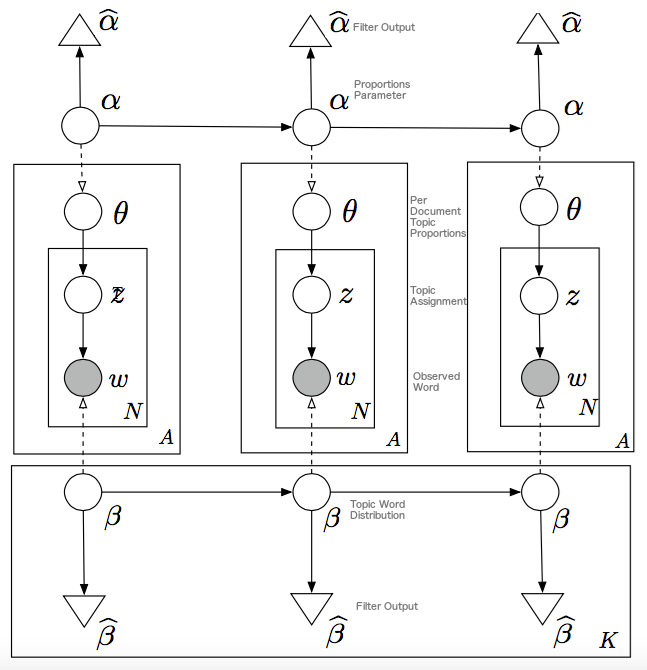
\includegraphics[width=130mm,scale=0.45]{Figures/DTMGM}
\caption[DTMGM]{Graphical model for DTM showing a series of chained static LDA models. The triangles represent the Kalman filter estimates of the hyper-parameters}
\label{fig:DTMGM}
\end{figure}

% could put in the new process from Blei here but maybe that's a bit too much like plagiarism? Would not be cool. 

\subsection{Variational approximate inference}
% motivating variational methods
Because we have used the Gaussian distribution to model the progression of our parameters, inference becomes intractable due to the non-conjugacy of Gaussian and multinomial models. To get around this we take the same variational approach to approximate inference as before in section \ref{ldaprimer} with static LDA. Taking a variational approach has the advantage of allowing us to handle larger document sets compared to Gibbs sampling which becomes computationally difficult at large corpus sizes. 

% variational methods
The general strategy of variational approximate inference is to use a carefully tuned 'approximate' distribution as a substitute for the true posterior. To tune this approximate distribution we minimize the KL divergence between our estimated and true posterior. Finally we may then use this approximated posterior distribution to perform inference.

We begin by creating a collection of variational parameters we will optimize over our latent variables. Our latent variables are the topics $\beta_{t,k}$, topic proportions $\theta_{t,d}$, and topic indicators $Z_{t,d,n}$. While we have variational parameters for each topic (consisting of a sequence of multinomial parameters), and for each document (the latent topic proportions). The resulting posterior, again following the notation of \parencite{Blei:2006:DTM:1143844.1143859} is given by equation \ref{eq:dtmpost}.

\begin{align*}
& \prod_{k=1}^K q(\beta_{k,1}, ... , \beta_{k,T} | \hat{\beta}_{k,1}, ... , \hat{\beta}_{k,T})  \times     \\
& \prod_{t=1}^T \Big( \prod_{d=1}^{D_t} q(\theta_{t,d})| \gamma_{t,d}) \prod_{n=1}^{N_{t,d}}q(z_{t,d,n}|\phi_{t,d,n})   \Big)  \numberthis \label{eq:dtmpost} 
\end{align*}

Now we are ready to tune our approximate posterior, and specifically the variational observations $\{ \hat{\beta}_{k,1}, ... , \hat{\beta}_{k,T}  \}$ according to the KL divergence between the estimated and the true posterior. Note that here, each topic proportions vector $\gamma_{t,d}$ receives a corresponding free Dirichilet parameter, while each topic indicator $z_{t,d,n}$ receives a corresponding free multinomial parameter $\phi_{t,d,n}$. To optimize the document topic proportion vectors we subsequently employ gradient ascent, however this is not necessary for the document level parameter updates as they simply have a closed form.

%topic tracking
Finally, we may track our variational parameters $\hat{\beta}$ and $\hat{\alpha}$  between time slices using either the Kalman filter or wavelet regression. For brevity we will not replicate the mechanics of these methods here and encourage the interested reader to refer to the derivations provided in detail in  \parencite{Blei:2006:DTM:1143844.1143859}.


%\subsection{Issues}
%The DTM is not without its fallbacks. 
%addresses several latent structures in the document collection such as topic evolution and prevalence, however does not address the birth and death of topics, like models such as \cite{DBLP:journals/corr/abs-1203-3463}.

%--------------------------------------------------------------------------------------
\section{DIM Model Overview} 
% Roadmap + Disclaimer
In this section we provide an overview of the Dynamic Influence Model (\keyword{DIM}) following closely the derivation found in \parencite{icml2010_GerrishB10}. For brevity, we do not replicate all technical aspects of the model here and encourage the interested reader to examine the original paper for a complete exposition of the mechanics of the DIM.

\subsection{DIM Purpose}
Aside from generating thematic topics, the unique purpose of the DIM is to provide estimates of document influences on each of those topics. The novelty of the DIM lies in the fact that this influence measure is inferred solely from language use. This makes the DIM particularly useful when traditional bibliometrics such as citations are unavailable, and in such cases inferred document influences could act as a proxy as the two are known to correlate \parencite{icml2010_GerrishB10}. The quantitative estimate of a document's influence that DIM provides is valuable as it allows for more informed decisions about publishing and funding, and can help us assign 'value' to documents in an automated manner. 

\subsection{Encoding Influence}
The DIM itself is a close relative to the DTM, as outlined above in section \ref{DTM}; it too consists of a series of individual LDA models connected via a Markov chain of term distribution parameters $\beta$. Naively we may describe the drift of this distribution as a stationary autoregressive process with transition variance $\sigma^2$, given by equation \ref{eq:naivechain}.

\begin{align*}
\beta_{t+1} | \beta_{t} \sim  \mathcal{N}(\beta_{t},\sigma^2I)
\numberthis \label{eq:naivechain}
\end{align*}

This in essence is the simplest form of the DTM, where we  compute the posterior distribution of our sequence of topics $\beta_{1:T}$ conditioned on the observed documents, and represent our corpus as a smooth trajectory of word frequencies.

However, with the DIM we wish to encode document influences into this model of topic drift. To do this we need a method of describing the probability of a word dependent on a set of natural parameters $\beta_t$. We write this probability as the softmax transformation of the unconstrained vector.

\begin{align*}
p(w|\beta_t) \propto exp(\beta_{t,w})
\end{align*}

Additionally, we assign to each document $d$ a normally distributed scalar influence score $\ell_d$ that describes the influence of that document on a given topic. Where a higher influence score indicates that a document's words had a larger impact on the drift of this topic. Finally, we modify our naive Markov chain of term distributions from equation \ref{eq:naivechain} to relate the next epoch's set of natural parameters $\beta_{t+1}$ to the probability of words under the \emph{current} set of natural parameters $\beta_t$, and the influence score of each document $\ell_d$.

\begin{align*}
\beta_{t+1} | \beta_t,(w,\ell)_{t,1:D} \sim  \mathcal{N}(\beta_t + exp(-\beta_t)\sum_dw_{d,t}\ell_{t,d},\sigma^2I)
\numberthis \label{eq:DIMchain}
\end{align*}

In this way, the words of a high influence document will have  a higher expected probability in the following time step. In effect, each topic's natural parameters are "nudged" by the words of each document in proportion to the influence score of that document. This is a core principle of the DIM, that not all documents exert the same force on the direction of a topic, some documents have a larger impact, a larger \emph{influence} on a given topic than others. As a result, an article whose words can help explain the way the word frequencies change will have a high posterior influence score.

Something is still missing though, equation \ref{eq:DIMchain} only expresses the progression of natural parameters for a single topic. For multiple topics we generalize this expression to equation \ref{eq:DIMchainmulti}, defining $z_{d,n,k}$ as the indicator that the nth word in document d is assigned to topic k.

\begin{align*}
\beta_{k,t+1} | \beta_{k,t},(w,\ell, z)_{t,1:D} \sim  \mathcal{N}(\beta_{k,t} + exp(-\beta_{k,t})\sum_d \ell_{d,k} \sum_n w_{d,n}z_{d,n,k},\sigma^2I)
\numberthis \label{eq:DIMchainmulti}
\end{align*}

Where to accommodate multiple topics we have kept the influence score of a document outside the summation over the possible indicator assignments. This yields the graphical model illustrated in figure \ref{fig:DIMGM}. If we compare this to the graphical model for the DTM present in figure \ref{fig:DTMGM} we can observe how the DIM differs. 

Particularly, we no longer chain our document topic-proportions $\alpha$ between time steps; instead each epoch's corresponding LDA receives the same set. Additionally the topic term-distribution hyper parameters of a given timestep $\beta_{t}$ depend not only the previous timestep's params $\beta_{t-1}$ but also the indicators $z$, terms $w$, and influences $\ell$ of the past timestep. Together these differences constitute a significant enough change to create a noticable difference in results between the DIM and DTM, which we report in Chapter \ref{Chapter4}.


\begin{figure}[ht]
\centering
\includegraphics[width=130mm,scale=0.45]{Figures/DIMGM}
\caption[DTMGM]{Graphical model of the DIM. Note the increased number of dependencies for the term distribution parameters $\beta$ compared to that of the DTM.}
\label{fig:DIMGM}
\end{figure}

\subsection{Inference with DIM}

Conducting inference with the DIM is largely similar to the DTM. Again, computing the exact posterior is intractable so we turn to variational methods to approximate it with a simpler distribution over latent variables. Here our latent variables are the sequence of topics and the per-document influence values, conditioned on an observed corpus. 

Our simple approximation of the true posterior is given by equation \ref{eq:DIMvardist}, which we call our \emph{variational distribution}. To specify this variational distribution we introduce a set of free variational parameters which we fit to minimize the KL divergence between the variational distribution and the true posterior. 

\begin{align*}
q(\beta, \ell, Z, \theta | \widetilde{\beta},  \widetilde{\ell}, \phi, \gamma) = \prod_{k=1}^k q(\beta_{k,1:T} | \widetilde{\beta}_{K,1:T}) \\
 \prod_{t=1}^T \prod_{d=1}^{D_{t}} q(\theta_{t,d} | \gamma_{t,d}) q(\ell_d | \widetilde{\ell}_d) \prod_{n=1}^{N_{t,d}} q(Z_{t,d,n} | \phi_{t,d,n})
 \numberthis \label{eq:DIMvardist}
\end{align*}

The first such variables we introduce include the word assignments $z_n$ and topic proportions $\theta_d$ which are governed by multinomial parameters $\phi_d$ and Dirichilet parameters $\gamma_d$. Additionally, in order to govern the variational distribution for topic trajectories $\{  \beta_{k,1},...,\beta_{k,T}  \}$, described by a linear gaussian chain, we specify the set of parameters $\{  \widetilde{\beta}_{k,1},...,\widetilde{\beta}_{k,T}  \}$ to act as the "variational observations" of the chain. Finally, in order to describe the variational distribution of the document influence value $\ell_{d,k}$ as a Gaussian we introduce $\widetilde{\ell}_{d,k}$ representing the mean, and $\sigma^2_{\ell}$ representing the fixed variance. 

Finaly, as stated above, we obtain estimates for these variational parameters by fitting our variational distribution, minimizing the KL divergence via gradient descent. It is here that we end our brief summary of the DIM. For more details such as parameter updates, and initial empirical results, we direct the interested reader to the full original exposition found in \parencite{icml2010_GerrishB10}.






















